%! TeX program = lualatex
\documentclass[../main.tex]{subfiles}
\begin{document} \section{Subtleties of extrema}
  Last week, we briefly talked about the Extreme Value Theorem.
  \begin{mdframed}[style=withref-compact]
    If \(f(x)\) is continuous over a closed and bounded interval \([a,b]\), then \(f\) must have an absolute maximum \hlsupp{and} an absolute minimum on \([a,b]\).

    \textbook{Theorem 4.1 Extreme Value Theorem on page 367}
  \end{mdframed}

  Why are the conditions \hlmain{continuous over a closed and bounded interval \([a,b]\)} in EVT necessary? Remember the examples on this page!

  \begin{example}
    Let \(f\) be a function defined over an interval \(I\) and consider the following scenarios. If one of the absolute extrema does not exist, then sketch a function satisfying the conditions in that row with no said absolute extrema.

    \begin{center}
      \begin{tabular}{p{1in}|l|p{4in}}
        \parbox{1in}{Continuous\\on \(I\)?} & \(I\) is \ldots{} & Has both absolute extrema? Why? \\ \midrule
        yes & closed and bounded & Yes, it has both extrema by EVT. \\\midrule
        \hlwarn{no} & closed and bounded & \\[1in] \midrule
        yes & closed but \hlwarn{not bounded} & \\[1in] \midrule
        yes & bounded but \hlwarn{not closed} & \\[1in]
      \end{tabular}
    \end{center}

    \faComment{} What if \(f\) is continuous and the \emph{range} of \(f\) is bounded? Is it enough to guarantee the existence of both absolute extrema? 

  \end{example}

  \medskip{}
  Let's consider a common misapplication of logic.
  \begin{example}
    The function \(f(x) = \frac{1}{x^{2} + 1}\) has no absolute minimum (Week 9, Example~\ref{ex:extremum-open-interval} on page \pageref{ex:extremum-open-interval}). Does this example contradict the Extreme Value Theorem? Explain your reasoning.
    \vfill{}
    \clearpage
  \end{example}

% \section{Subtleties of the Derivative Tests}
%   Now we discuss subtleties of the derivative tests. We discuss the local maximum case in class and leave the local minimum case as exercises.
%
%   The First Derivative Test is very \underline{\hspace{3cm}} about the sign change. To certify a local maxima at a critical number \(c\), the First Derivative Test asks us to show that the sign of \(f'\) changes
%   \blanklines{3}
%
%   Why can't we relax the sign-change to
%   \blanklines{3}
%
%   We have to really unpack the statement of the First Derivative Test to figure out the reason. 
%
%   \begin{example}
%     Notice \(f\) can be applied to a critical number \(c\) at which \(f'(c)\) \underline{\hspace{2in}}, then the following situation can happen, for example, at the critical number \(c = 0\).
%
%   \[
%     f_{1}(x) = 
%     \begin{cases} 
%       x^{3} + 1/4 & \text{if } x \le 0 \\ 
%       1/4& \text{if } x > 0
%     \end{cases}
%     \qquad
%     f_{2}(x) = 
%     \begin{cases} 
%       x^{3} + 1/4 & \text{if } x \le 0 \\ 
%       1/2& \text{if } x > 0
%     \end{cases}
%   \]
%   \quad
%   \begin{center}
%     \begin{tikzpicture}
%       \begin{axis}[ymin=-1, ymax=1, xmin=-1, xmax=1, width=2in, xtick={-1,0,1}, ytick={-1,0,1}, title={\(f_{1}(x)\)}, ylabel={}]
%         \addplot[ultra thick, domain=-1:0] {x^3+1/4};
%         \addplot[ultra thick, domain=0:1] {1/4};
%         \draw[warn, fill=warn] (axis cs:0,1/4) circle[radius=2pt];
%       \end{axis}
%     \end{tikzpicture}
%     \quad
%     \begin{tikzpicture}
%       \begin{axis}[ymin=-1, ymax=1, xmin=-1, xmax=1, width=2in, xtick={-1,0,1}, ytick={-1,0,1}, title={\(f_{2}(x)\)}, ylabel={}]
%         \addplot[ultra thick, domain=-1:0] {x^3+1/4};
%         \addplot[ultra thick, domain=0:1] {1/2};
%         \fill (axis cs:0,1/2) circle[radius=2pt];
%         \draw[fill=white] (axis cs:0,1/2) circle[radius=2pt];
%         \draw[warn, fill=warn] (axis cs:0,1/4) circle[radius=2pt];
%       \end{axis}
%     \end{tikzpicture}
%
%     \begin{tikzpicture}
%       \begin{axis}[ymin=-1, ymax=1, xmin=-1, xmax=1, width=2in, xtick={-1,0,1}, ytick={-1,0,1}, title={\(f'_{1}(x)\)}, ylabel={}]
%         \addplot[ultra thick, domain=-1:0] {x^2};
%         \addplot[ultra thick, domain=0:1] {0};
%       \end{axis}
%     \end{tikzpicture}
%     \quad
%     \begin{tikzpicture}
%       \begin{axis}[ymin=-1, ymax=1, xmin=-1, xmax=1, width=2in, xtick={-1,0,1}, ytick={-1,0,1}, title={\(f'_{2}(x)\)}, ylabel={}]
%         \addplot[ultra thick, domain=-1:0] {x^2};
%         \addplot[ultra thick, domain=0:1] {0};
%         \draw[fill=white] (axis cs:0,0) circle[radius=2pt];
%       \end{axis}
%     \end{tikzpicture}
%   \end{center}
% \end{example}
%
%   Let's use the above quirkiness to understand the ability of the First Derivative Test. 
%   \begin{example}
%     The function \(f_{1}\) and \(f_{2}\) above both have infinitely many local max on the interval \((0,1)\). Is it possible to detect these local maximum by applying the First Derivative Test?
%   \end{example}
%
% 
\section{Sketching using derivatives}
  We know how to sketch the graph of a function by transforming the graph of certain basic functions.  This technique works for sufficiently simple function, but not complex functions. The good news is that we can use derivative tests and asymptotes to sketch the graph of many more function.

  The following two pictures tell us everything about mixing increasing/decreasing and concavity.
  \begin{center}
    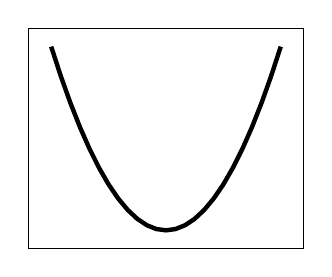
\begin{tikzpicture}
      \begin{axis}[width=2in, xtick=\empty, ytick=\empty, xlabel={}, ylabel={}]
        \addplot[ultra thick, domain=-1:1] {x^2};
      \end{axis}
    \end{tikzpicture}
    \hspace{1in}
    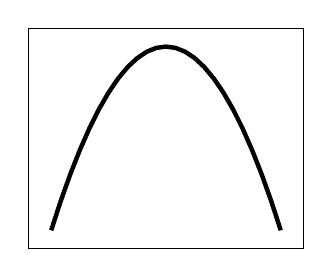
\begin{tikzpicture}
      \begin{axis}[width=2in, xtick=\empty, ytick=\empty, xlabel={}, ylabel={}]
        \addplot[ultra thick, domain=-1:1] {-x^2};
      \end{axis}
    \end{tikzpicture}
  \end{center}
  \blanklines{5}

  \begin{example}
    Sketch the graph of a function \(f(x)\) satisfying the following properties.
    \begin{itemize}
      \item \(f\) is defined and continuous on \((-1, \infty)\).
      \item \(\lim_{x \to -1^{+}} f(x) = -\infty\).
      \item \(\lim_{x \to \infty} f(x) = 3\).
      \item \(f\) is increasing over the interval \((-1,\infty)\).
      \item \(f\) is concave down on the interval \((-1,1)\).
      \item \(f\) is concave up on the interval \((2, 3)\).
      \item \(f\) has inflection points at points \((1,1)\) and \((2,2)\).
    \end{itemize}

    \blanklines{15}
  \end{example}

\end{document}
